\section{Results}
% Beskriv omstændigheder, fysiske rammer og program versinoer etc,
% samt hvordan resultaterne er genereret.

The following images were all generated on the same machine, using the
current\footnote{2013-12-09} version of the DSC mesh structure, Chan-Vese
segmentation implementation and my visMesh plugin. The machine is a modern i7
based computer with 24GB RAM running Maya 2013 on Windows 8.

\subsection{Testing the CMake Build}
The purpose of using CMake was to ease the process of building projects and
compiling the plugin on different platforms. During the meetings the plugin was
compiled on one of the supervisors MacBook and during daily development I
compiled it on Windows 7 and 8 using both Visual Studio 2010 and 2012. The path
to the DSC project needs to be changed for each machine as described in Section
\ref{sec:cmake}.

\subsection{visMesh \& OpenGL Solution}
First lets take a look at the original implementation, it spawns an OpenGL
window as seen in Figure \ref{fig:OpenGLwindow}.

\graphicc{1.0}{img/openglwindow.png}{The current OpenGL based visualization
program immediately after it is launched.}{fig:OpenGLwindow}

The program expects you to know the keyboard shortcuts and mouse usage in order
to simulate or move the camera, it can display only one material with a static
illumination. The ``segmentation'' of the \textit{cube\_coarse.dsc} file can be
seen in four different stages in Figure \ref{fig:OpenGL}. The settings for the
simulation and the startup file cannot be changed without recompiling the
program.

\begin{figure}
        \centering
        \begin{subfigure}[t]{0.4\textwidth}
                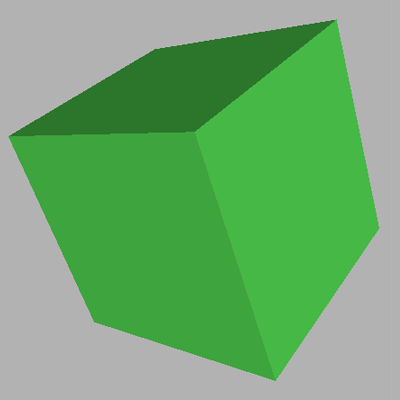
\includegraphics[width=\textwidth]{img/gl0.png}
                \caption{The initial cube with no simulation steps.}
                \label{fig:gl0}
        \end{subfigure}%
        ~ % use \qquad??
        \begin{subfigure}[t]{0.4\textwidth}
                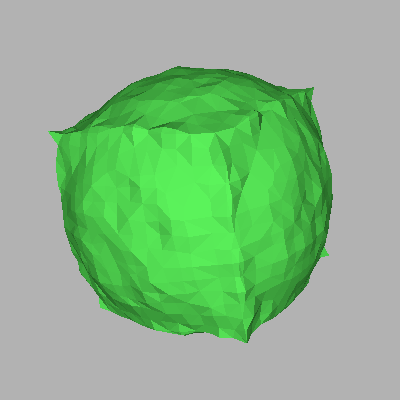
\includegraphics[width=\textwidth]{img/gl1.png}
                \caption{The cube after some simulation steps. The sides have
                         startet to ``bulge'' as the simulator begins to move
                         vertices towards a spherical shape.}
                \label{fig:gl1}
        \end{subfigure}

        \begin{subfigure}[t]{0.4\textwidth}
                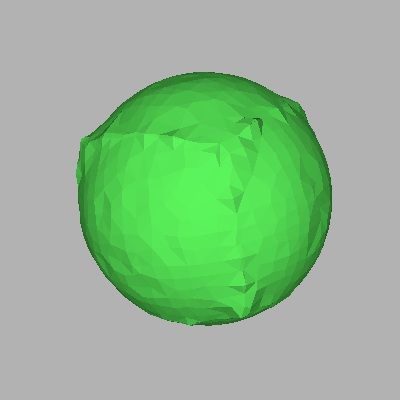
\includegraphics[width=\textwidth]{img/gl2.png}
                \caption{Towards the end, the cube looks more like a sphere with
                         eight pinched corners.}
                \label{fig:gl2}
        \end{subfigure}%
        ~ % use \qquad??
        \begin{subfigure}[t]{0.4\textwidth}
                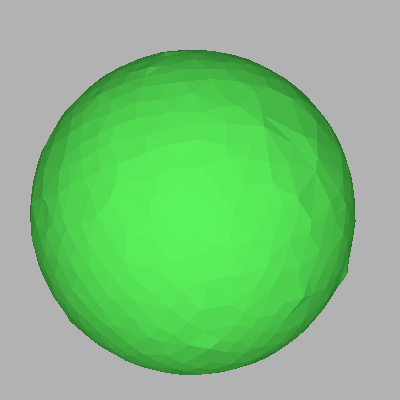
\includegraphics[width=\textwidth]{img/gl3.png}
                \caption{At this point, the cube is as spherical as it will get,
                         the vertices moves around a little, but the overall
                         shape do not change.}
                \label{fig:gl3}
        \end{subfigure}
        \caption{Pictures of four different stages in the simulation process using
                 the current OpenGL based simulation/visualization tool.}
        \label{fig:OpenGL}
\end{figure}

The result of running the simulation as in Figure \ref{fig:OpenGL}with the same
settings\footnote{Sphere radius: $0.25$ and step size: $0.01$.} in the visMesh
plugin will yield the results shown in Figure \ref{fig:vismesh}.

\begin{figure}
        \centering
        \begin{subfigure}[t]{0.4\textwidth}
                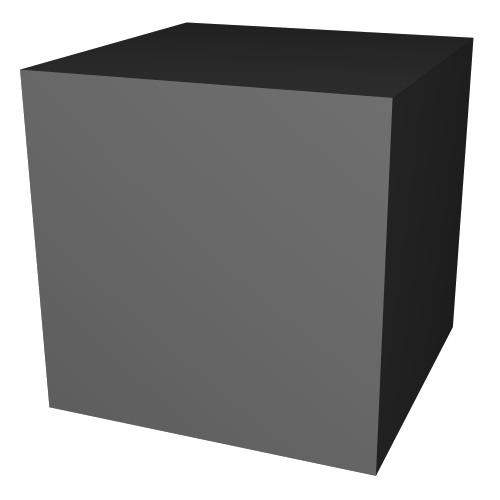
\includegraphics[width=\textwidth]{img/maya0.png}
                \caption{The initial cube with no simulation steps.}
                \label{fig:Maya0}
        \end{subfigure}%
        ~ % use \qquad??
        \begin{subfigure}[t]{0.4\textwidth}
                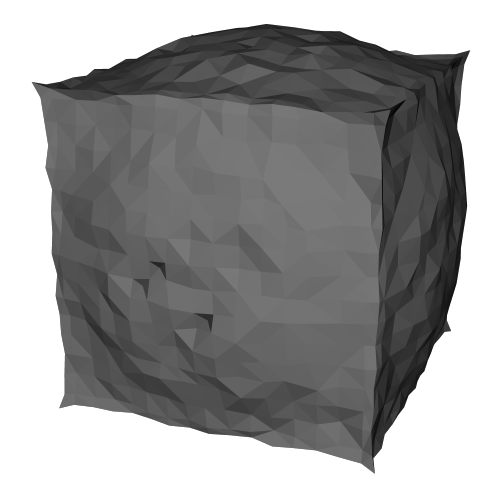
\includegraphics[width=\textwidth]{img/maya1.png}
                \caption{The cube after some simulation steps. The sides have
                         started to ``bulge'' as the simulator begins to move
                         vertices towards a spherical shape.}
                \label{fig:Maya1}
        \end{subfigure}

        \begin{subfigure}[t]{0.4\textwidth}
                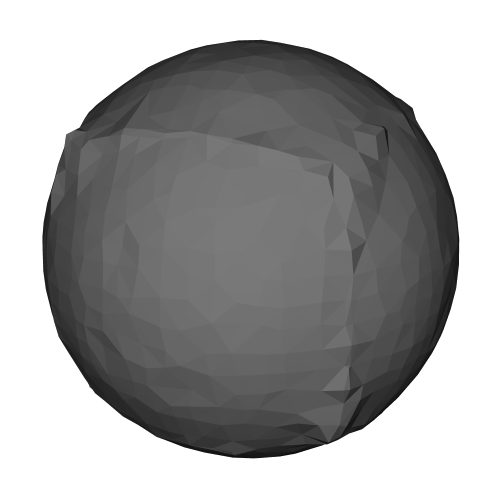
\includegraphics[width=\textwidth]{img/maya2.png}
                \caption{Towards the end, the cube looks more like a sphere with
                         eight pinched corners.}
                \label{fig:Maya2}
        \end{subfigure}%
        ~ % use \qquad??
        \begin{subfigure}[t]{0.4\textwidth}
                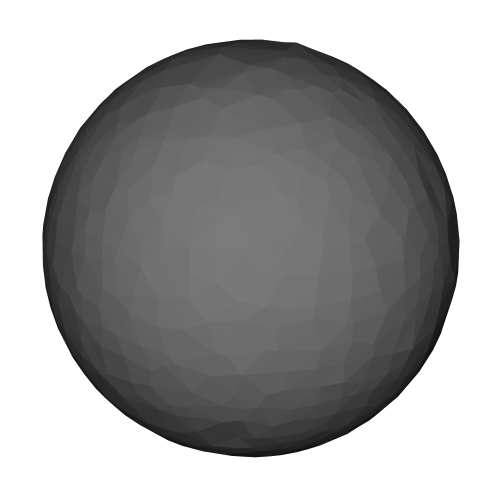
\includegraphics[width=\textwidth]{img/maya3.png}
                \caption{At this point, the cube is as spherical as it will get,
                         the vertices moves around a little, but the overall
                         shape do not change.}
                \label{fig:Maya3}
        \end{subfigure}
        \caption{Pictures of four different stages in the simulation process using
                 the visMesh plugin.}
        \label{fig:vismesh}
\end{figure}

As seen in Figure \ref{fig:vismesh} the simulation performed is the same and
gives the same results, showing that the segmentation code still works under my
plugin without distorting the results.

When the plugin is loaded and a proper node is created (see section
\ref{sec:melsetup}) it will spawn a $1\times 1\times 1$ cube with Mayas default
material and shader, it will look like Figure \ref{fig:defaultmesh}.

\graphicc{0.5}{img/defaultmesh.png}{The default mesh spawned by the plugin if no
mesh file has been specified. Note that the above screenshot has the viewport
set to softshading.}{fig:defaultmesh}

When the plugin node is selected, the options given by the simulator class
will be visible along with a way of selecting an initialization file. The number
of parameters visible depends on what the simulator responds via the
\texttt{getArguments()} method. As seen in Figure \ref{fig:args} it can be any
number of parameters, but if the name of the parameter is too long, it will be
hidden unless the pane it belongs in gets expanded. Figure \ref{fig:args0}
show the settings for a simulator I implemented, it translates a cube along the
x-axis. Figure \ref{fig:args1} are the settings the Chan-Vese simulation.

\begin{figure}
        \centering
        \begin{subfigure}[b]{0.48\textwidth}
                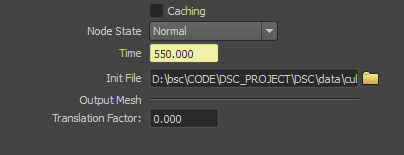
\includegraphics[width=\textwidth]{img/args0.png}
                \caption{The parameters for a translation simulator I created
                         for testing the plugin.}
                \label{fig:args0}
        \end{subfigure}%
        \hspace{10px} % use \qquad??
        \begin{subfigure}[b]{0.48\textwidth}
                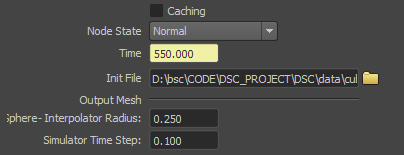
\includegraphics[width=\textwidth]{img/args1.png}
                \caption{The parameters for the Chan Vese simulation class.}
                \label{fig:args1}
        \end{subfigure}
        \caption{Pictures of the parameters pane for the plugin using different
                 simulators.}
        \label{fig:args}
\end{figure}

Clicking the ``folder icon'' in the parameter pane will let you select a mesh
file via a dialog box used to start the simulator. Currently, the Chan Vese
simulator class I have written will load any DSC mesh as long as the file is
properly structured since it uses the existing DSC library to load the mesh.
To test this, apart from loading the \textit{cube\_coarse.dsc}, I also tried to
load \textit{cube\_fine.dsc} and \textit{bunny.dsc}.

Loading the cubes works fine, a mixed image of both can be seen in figure
\ref{fig:cube-mix}. A picture of the bunny in wireframe and with a
smoothshader under the wireframe is mixed in Figure \ref{fig:bunny-mix}.

\graphicc{0.6}{img/cube-mix.png}{The fine and coarse cube mashed into one
image.}{fig:cube-mix}
\graphicc{0.6}{img/bunny-mix.png}{The bunny DSC file loaded into Maya and viewed
in wireframe mode and with a smoothshader under the wireframe.}{fig:bunny-mix}

One of the benefits of the plugin is that it is easy to define new materials even
if they are pretty advanced. Figure \ref{fig:gradients} shows three different
meshes with a gradient shader that changes color depending on the angle of the
light source.

\begin{figure}
        \centering
        \begin{subfigure}[t]{0.3\textwidth}
                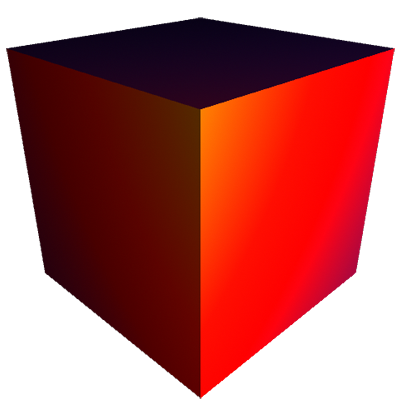
\includegraphics[width=\textwidth]{img/gradientmat0.png}
                \caption{The corase cube with a gradient shader.}
                \label{fig:gradientmat0}
        \end{subfigure}%
        ~ % use \qquad??
        \begin{subfigure}[t]{0.3\textwidth}
                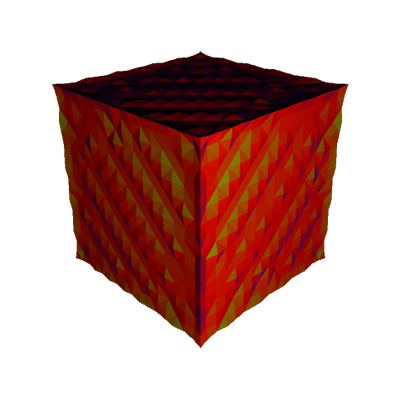
\includegraphics[width=\textwidth]{img/gradientmat1.png}
                \caption{The coarse cube after 200 steps of the Chan Vese
                         simulation with a low radius.}
                \label{fig:gradientmat1}
        \end{subfigure}
        ~ % use \qquad??
        \begin{subfigure}[t]{0.3\textwidth}
                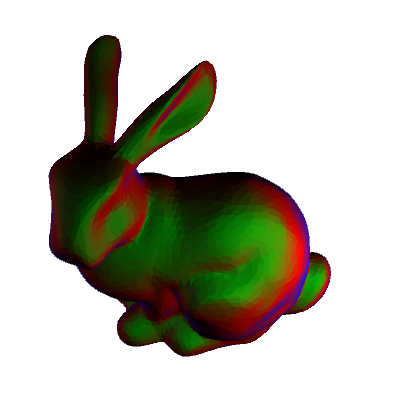
\includegraphics[width=\textwidth]{img/gradientmat2.png}
                \caption{The bunny with the same shader as the cubes.}
                \label{fig:gradientmat2}
        \end{subfigure}

        \caption{The gradient shader used in the images above go between red,
                 blue and green depending on the angle the light hits it.}
        \label{fig:gradients}
\end{figure}

Since the mesh does not provide UV-mapping information I am unable to use 2D
textures such as bitmaps as materials since Maya does not by default know how to
apply the texture. The generic textures with highlights and transparency
will work perfectly with the plugin.

The ability to easily use custom textures and look at wireframe-renders means
that it is easier to inspect the mesh, look for errors in the mesh structure,
or to make sure that a simulator does what it is supposed to. A limitation is
that it only renders surfaces, it is not possible to look inside the mesh and
check if the inner tetrahedrons are properly formed.

It is possible to let Maya count the number of faces and vertices both in the
total scene, the selected object and the selected sub-area. An example of the
count for the bunny mesh can be seen in figure \ref{fig:meshinspect}.

\graphicc{1.0}{img/meshinspection.png}{This is the bunny mesh with smooth
          shading and a wireframe look. In the upper left corner the mesh
          information for the scene and mesh itself is visible. Note that the
          UV count is 0 because there is no UV information in the mesh, and the
          face and tri counts are the same because DSC only contains triangle
          faces.
          The coloumns of numbers represent the total number in the scene, the
          number in the selected object and the number on the selected
          subobject.}
          {fig:meshinspect}

To test the plugins ability to function as an animation tool, I created
three animations using Maya:
\begin{itemize*}
  \item An animation where the analytical cube is interpolated to a small
    sphere, using the default Lambert shader from Maya:
    \myurl{http://www.youtube.com/watch?v=MFQexA6nB8Q}

  \item An animation using the same parameters as the OpenGL application, using
    a Lambert shader that have been ``whitened'' to test how the plugin handles
    different shader parameters:
    \myurl{http://www.youtube.com/watch?v=w3XM847AqOk}

  \item Same simulation as above, but with a rotation animation on the final
    mesh to test if transformations will work properly, a ramp shader have also
    been applied that changes color depending on the angle it's viewed from:
    \myurl{http://www.youtube.com/watch?v=H8yS482NGbI}
\end{itemize*}

%TODO: Add a wrap up on the movies here.

\subsection{Performance}
In order to get an idea of the performance of the visMesh plugin, I ran the
segmentations of the \textit{cube\_coarse.dsc} and \textit{cube\_fine.dsc} files
through visMesh and the OpenGL application. I noted down both the CPU and memory
usage of both methods during segmentation and when just ``watching'' the
geometry.

I had no way of making accurate measurements for how long a segmentation
timestep takes under visMesh and the OpenGL application respectively. But a
rough timing by running them side by side show a similar performance. This is a
very crude measurement, so I will refrain from making any conclusions based on
this data.

When performing the segmentation itself, the CPU usage for both the OpenGL
application and the visMesh plugin is very similar, they both use around 13-15\%
CPU when segmenting (on both cubes). Based on the console output most of the
time is spend by the DSC framework to optimize the mesh. The 13-15\% usage
corresponds to one full CPU core on my machine. So if the DSC framework could be
made to use several cores I believe that both the OpenGL application and visMesh
would gain performance. When just displaying the mesh, the OpenGL application
used 7-0\% CPU to display the coarse cube, and 15\% to display the fine cube.
With the fine cube there was also a significant FPS\footnote{\textit{Frames Per
Second} - How fast a display(-port) updates its image.} drop in the OpenGL
application. visMesh would use 13-15\% CPU when segmenting, just like the OpenGL
application. When displaying the mesh itself, visMesh uses Mayas optimized
rendering engine and would use between 0-2\% CPU with both cubes and there is no
loss of framerate when viewing the fine cube.

Memory wise there is a huge difference between visMesh and the OpenGL
application. While the OpenGL application only stores the current mesh, visMesh
will store all of the meshes it have simulated so far. With this test I wanted to
assess two things, how much memory does the mesh take up in visMesh, and how
much does it take up in the OpenGL application.

My raw numbers can be found in Appendix
\ref{sec:benchmarks}. When the coarse cube is loaded in the OpenGL application,
it uses \~65MB of memory. The fine cube takes \~392MB of memory. This memory is
the total of what is used by the ChanVese code in memory, the DSC code and data
in memory and the OpenGL renderer.\footnote{Due to the FPS-drop earlier I assume
it is rendering using the CPU rather than the GPU since there was no load on my
GPU during the benchmark.} When the cubes are loaded in memory Maya takes up
318MB for the coarse cube and 641MB for the fine. This is significantly higher
than the OpenGL application, but it includes all of Mayas runtime code. In order
to determine how much memory the plugin itself uses we should deduct how much
memory Maya uses by itself. Launching Maya a number of times and looking at the
memory use once everything but visMesh is loaded shows Maya have an approximate
memory use of 257MB. This gives a visMesh memory use of 61MB and 384MB for the
cubes. This memory includes the DSC own mesh storage used by the simulator (the
most recent mesh) and the mesh displayed in frame 0 of the simulation.

These numbers show a slightly smaller memory footprint for two meshes in visMesh
than a single mesh in the OpenGL application. When the simulation goes on, the
memory of the OpenGL application does not increase as it only stores one mesh at
any time but is unable to rewind. visMesh will store all the meshes so it's
memory footprint will increase for each frame simulated. For the cube
segmentation the mesh becomes slightly less complicated over time, as the size
decrease and DSC removes superfluous tetrahedrons. This yields a $O(f\cdot c)$
memory footprint for visMesh, where $f$ is the number of frames, and $c$ is the
complexity of the most complex mesh stored. In order to test this hypothesis I
ran two 1000 frame simulation using the default simulator values. The
simulations were the segmentation of the fine and coarse cubes.

\begin{figure}
        \centering
        \begin{subfigure}[t]{1\textwidth}
                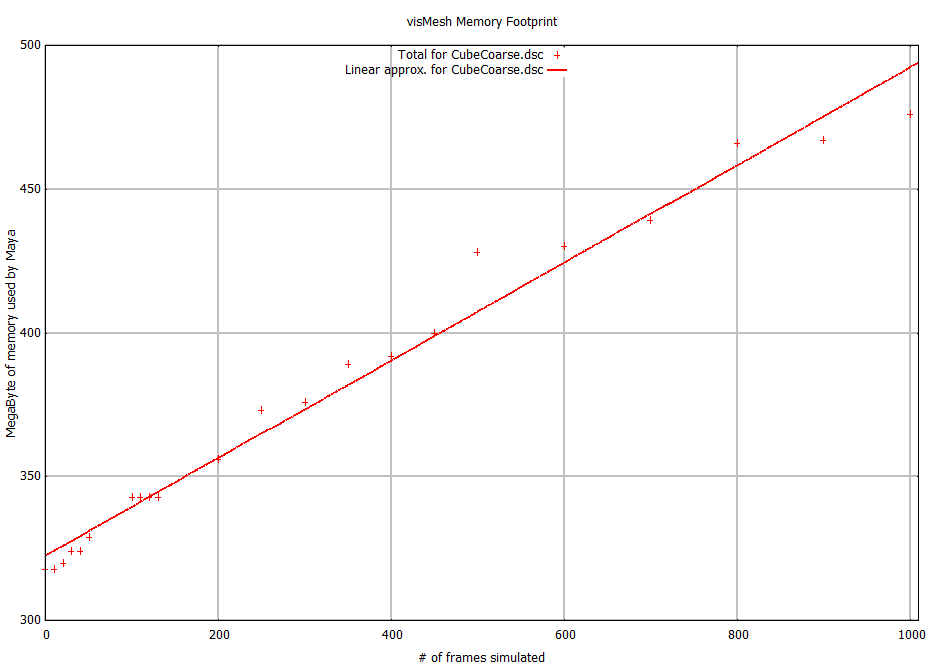
\includegraphics[width=\textwidth]{img/cubeCoarse-graph.png}
                \caption{Memory use of Maya over a 1000 frame segmentation of
                the coarse cube.}
                \label{fig:memorycoarse}
        \end{subfigure}%
\\
        %~ % use \qquad??
        \begin{subfigure}[t]{1\textwidth}
                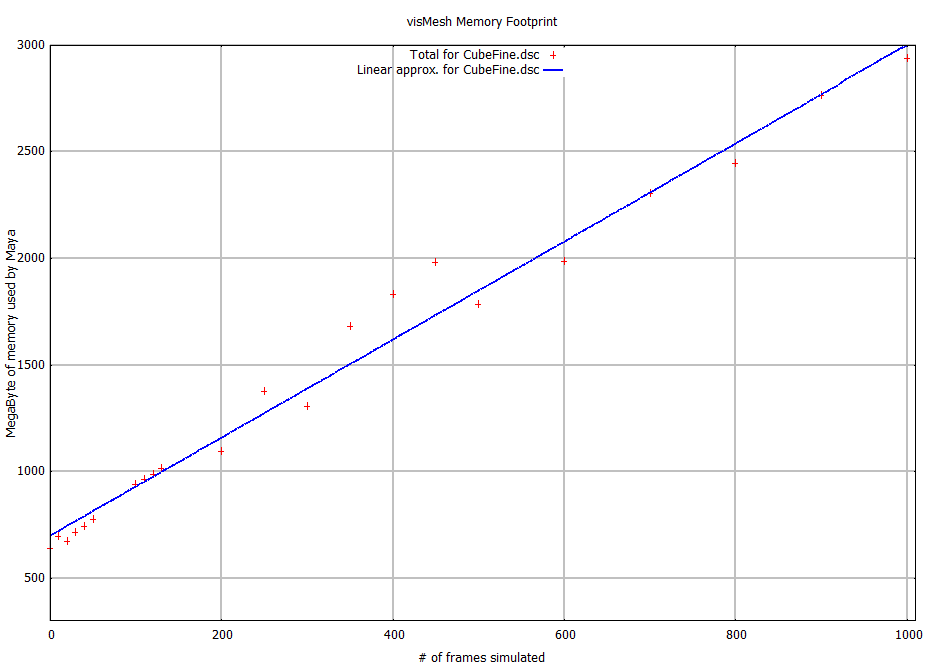
\includegraphics[width=\textwidth]{img/cubeFine-graph.png}
                \caption{Memory use of Maya over a 1000 frame segmentation of
                the fine cube.}
                \label{fig:memoryfine}
        \end{subfigure}

        \caption{Graphs and trendlines for the memory use of two different
        segmentations using the visMesh plugin including Mayas own memory use.}
        \label{fig:membenchmarks}
\end{figure}

Figure \ref{fig:membenchmarks} shows the results of monitoring the memory use
as the simulation progresses. Trend lines have been laid in that was fitted
using GNU plot in order to see if the recorded memory usage would line up
with/below the expected linear $O(f\cdot c)$ usage. Both Figure
\ref{fig:memorycoarse} and Figure \ref{fig:memoryfine} are grouped nicely around
the trend lines. The linear approximations are based on the data points
themselves so it will go roughly through the ``middle'', the test is to see if
any points stray too far (on the y-axis) from the line, indicating an unexpected
higher memory use.

On both graphs there is a few points (See \ref{fig:memorycoarse} frame 500 and
1000) that strays a bit far. I am unable to explain exactly why this is. Based
on the fact that it happens several times, and that the memory increases,
then is steady for several points would suggest that it is the memory allocation
for Mayas array datatypes that causes these jumps.

% Write something about the memory footprint and maybe calculation times?
% Can the overhead be measured?
% Take Maya memory with empty scene, subtract that from the memory load when
% 100 frames have been simulated.
% Do a graph of the memory usage, should be linear or below (in my example the mesh gets simpler and simpler (cube->sphere)
% Compare to the footprint of the OpenGL app.
% Current limiting factor, speed per core (since nothing is threaded)